\documentclass{article}
\usepackage{graphicx}
\usepackage{amsmath}
\usepackage{float}
\usepackage{color}
\usepackage{calc}
\newsavebox\CBox
\newcommand\hcancel[2][0.5pt]{%
  \ifmmode\sbox\CBox{$#2$}\else\sbox\CBox{#2}\fi%
  \makebox[0pt][l]{\usebox\CBox}%  
  \rule[0.5\ht\CBox-#1/2]{\wd\CBox}{#1}}

\begin{document}
\section{Chapter 1}
\subsection{Exercises}
\subsubsection{Question 1.2}
\textbf{(a)} Absolute error $\approx 0.141592653$, the relative error $\approx 
4.507$ \%.


\textbf{(b)} Absolute error $\approx 0.001592653$, the relative error $\approx 
0.0506957$ \%.


\textbf{(c)} Absolute error $\approx 0.001264489$, relative error $\approx 
0.0402499$ \%.

\subsubsection{Question 1.5}

The condition number is defined as follows:
$$Cond = \frac{|(f(\hat{x}) - f(x))/f(x)|}{|(\hat{x}-x)/x|}$$

but more carefully:
$$Cond = \frac{|((x + \Delta x)-(y + \Delta y)) - \textcolor{blue}{(x-y)}|/|
\textcolor{red}{x-y}|}{|(|x + \Delta x| + |y + \Delta y|)-(\textcolor{blue}{|x| + 
|y|})|/(\textcolor{red}{|x| + |y|)}}$$
$$\geq \frac{|(\hcancel{(x - y)}\textcolor{blue}{\epsilon} + \Delta x - \Delta y) 
- \textcolor{blue}{\epsilon}|/|\textcolor{red}{\epsilon}|}{|(\hcancel{|x| - |x|} + 
|\Delta x| + \hcancel{|y | - | y|} + \Delta y|)|/(\textcolor{red}{1})}$$

$$ = \frac{|\Delta x - \Delta y| /\epsilon}{(|\Delta x| + |\Delta y|)/1} $$
$$ \geq \frac{1}{\epsilon} $$

The condition number is therefore necessarily larger than $\frac{1}{\epsilon}$, 
which means as $\epsilon$ gets closer to 0, we have more sensitivity in $f$. Since 
$x-y \approx \epsilon$, this means that the function gets more sensitive the 
closer $x$ and $y$ are to each other in value.

\subsubsection{Question 1.6}
Forward error is $\hat{f}(x)-f(x)$, and the backward error is $\hat{x} - x$ where 
$f(\hat{x}) = \hat{f}(x)$.


\textbf{(a)}

\textit{x=0.1}: The forward error is $$0.1 - sin(0.1) = 1.665*10^{-4},$$
the backward error is $$\hat{x} -x = sin^{-1}(0.1) -0.1 = 0.100167 - 0.1 = 
1.67*10^{-4}.$$


\textit{x=0.5}: The forward error is $$0.5 - sin(0.5) = 0.0205,$$ the backward 
error is
$$\hat{x} -x = sin^{-1}(0.5) - 0.5 = 2.36 * 10^{-2}.$$


\textit{x=1.0}: The forward error is $$1 - sin(1) = 0.1585,$$ and the backward 
error is $$\hat{x}-x=sin^{-1}(1) - 1 = 0.5708.$$

\textbf{(b)}
In this case, the forward error is $$\hat{f}(x) - f(x) = x-\frac{x^{3}}{6} - 
sin(x),$$
and the backward error can be found using the following:
$$backerr = \hat{x} - x,$$
where

$$\hat{x} = f^{-1}(\hat{f}(x)) = arcsin(x - \frac{x^{3}}{6}),$$

\textit{x=0.1}: The forward error is $$0.1-\frac{(0.1)^{3}}{6} - sin(0.1)= 
-8.331*10^{-8},$$ and the backward error is $$x - \hat{x} = 0.1 - arcsin(0.1 - 
\frac{0.1^3}{6} = 0.000000083731.$$

\textit{x=0.5}: The forward error is $$0.5-\frac{(0.5)^{3}}{6} - sin(0.5)= 
-2.588*10^{-4},$$  and the backward error is $$x - \hat{x} = 0.5 - arcsin(0.5 - 
\frac{0.5^3}{6} = 0.00029495.$$

\textit{x=1.0}: The forward error is $$1.0-\frac{(1.0)^{3}}{6}- sin(1.0) = 
-8.137*10^{-3},$$ and the backward error is $$x - \hat{x} = 1.0 - arcsin(1.0 - 
\frac{1.0^3}{6} = 0.0148892.$$

\subsubsection{Question 1.10}

\paragraph{\textbf{(a)} For x values near 0.}
\paragraph{\textbf{(b)} The following is more stable around x = 0 
because any 
rounding errors only occur once.
$$\frac{1}{1-x} - \frac{1}{1+x} = \frac{2x}{1- x^2}$$}


\subsubsection{Question 1.22}
Assume a normalized floating-point system with $\beta{} = 10$, $t = 3$, 
and
$L = -98$.

\paragraph{(a)}
$$UFL = \beta{}^{l} = 10 ^{-98}$$

\paragraph{(b)} If $x = 6.87 × 10^{-97}$ and $y = 6.81 × 10^{-97}$ ,
what is the result of $x - y$?\\

Ignoring the system, $x - y = 0.06 * 10 ^{-97}$ which if we normalize 
(which in 
the initial case we must), we have the result = $6*10^{-99}$ which is 
smaller than 
the underflow value. If we're assuming truncation, then we end up with 
a value of 
0 for this result.



\paragraph{(c)}What would be the result of $x - y$ if the
system permitted gradual underflow?

If the system permitted gradual underflow, then the result would be

$$result= 0.60 * 10^{-98}.$$


\subsection{Computer Exercises}
\subsubsection{Question 1.6}

\textbf{(a)}The method which uses multiplication, ie

$$x_k = a + kh, \qquad k=0,...,n$$

is better than the recursive summation method. Since we are using 
floating
point arithmetic, every step of the recursive method will involve some 
rounding. 
This loss of precision (error) will accumulate in the sum. While the 
multiplicative method also involves rounding, there are only two 
opperations, so 
the loss of precision is restricted to whatever occurs because of those 
two 
operations. Basically there are two rounding errors for the 
multiplicative method 
while the recursive method adds $n$ rounding errors.

\textbf{(b)}
In order to do this we set $a=0$, $b=1$ and use $n=10000$. We computed 
the $x_k$ 
for both methods and compared the results by taking the squared error 
between each 
term of each method and a true set of values achieved using 
$np.linspace$. The 
code can be found in $assignment1.ipynb.$\\

\begin{figure}[H]
	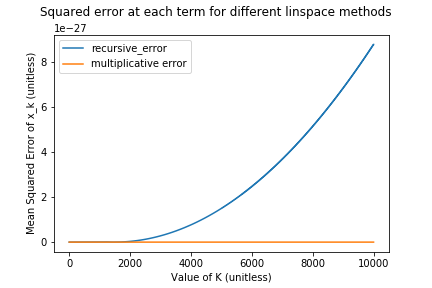
\includegraphics[width=\textwidth]{fig_ch1_cp1_6.png}
	\label{fig:ch1_cp1_6}
	\caption{Comparison of the error of the two proposed linspace generation 
	methods.}
\end{figure}

\subsubsection{Question 1.7}

\begin{figure}[H]
	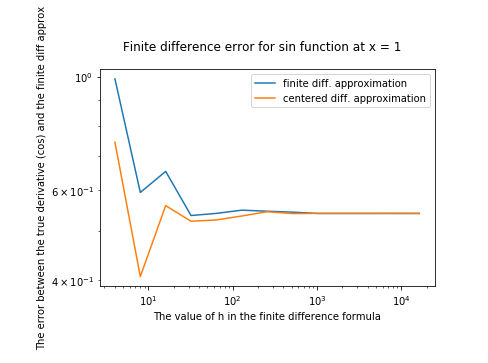
\includegraphics[width=\textwidth]{finite_diff_error_plot.png}
	\label{fig:ch1cp17}
	\caption{Plot of the errors for the finite difference and centered
	 difference approximations of the derivative of sin(x) at x = 1.0
	  for different values of h.}
\end{figure}

There isn't really much to comment about for this question. The plot 
requested can be found in figure \ref{fig:ch1cp17}. Appart from that 
you can find the code in $assignment1.ipynb.$\\




\subsubsection{Question 1.9}

\paragraph{(a)} The code for this question can be found in 
$assignment1.ipynb.$

\paragraph{(b)} The natural way to stop is when the term we are adding 
hits the value of 0. This is because factorials grow faster than their 
equivalent polynomials, so at one point the denominator will be so much 
bigger than the numerator that it will round to zero in the computer.

\paragraph{(c)} The results are shown in figure \ref{fig:q19}


\begin{figure}[H]
	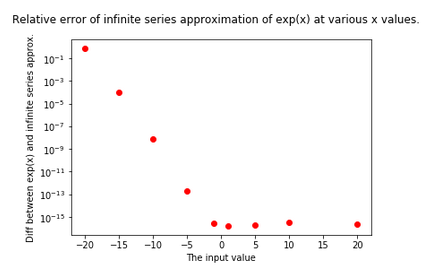
\includegraphics[width=\textwidth]{exp_infinite_series.png}
	\label{fig:q19}
	\caption{Plot of the relative error of the infinite series 
	approximation
	of the exponential function.}
\end{figure}

\subsubsection{Question 1.10}
The code for this question can be found in assignment1.ipynb.

The explanations for implementation are commented into the code.
Effectively, the first step was to check for a linear equation,
that is, if the $a$ coefficient is effectively zero. If this is
the case, then we have a linear equation. If the $b$ coefficient
is non-zero the we have a single root. If the $b$ coefficient is
also zero, then our fuction is a constant and it has no roots.


The next thing to check is to see if there are any imaginary roots.
If there are we don't handle them, because we are told not to in the
question spec.


Next we check if the square root of the discriminant is negligible
(i.e. smaller than the machine epsilon). If it is then we have a
repeating root case.

Finally, if all of those pass, then we need to select the standard
and alternate methods for each root in order to avoid cancelation in the
$b$ coefficient and the determinant. This involves picking the formula
which matches the sign for the two for each root.


Any further details can be found in the code. The results for the test
cases are given bellow:

\begin{center}
\begin{tabular}{| c c c || c | c|}
\hline
a & b & c & $1^{st}$ root & $2^{nd}$ root \\
\hline
6 & 5 & -4 & 0.5 & -1.3333333333333333\\
6e+30 & 5e+30 & -4e+30 & 0.5 & -1.3333333333333335\\
0 & 1 & 1 & -1.0 & nan\\
1 & -100000.0 & 1 & 99999.99999 & 1.0000000001000001e-05\\
1 & -4 & 3.99999999 & 2.000099999999696 & 1.999900000000304\\
1e-30 & -1e+30 & 1e+30 & 1.0 & nan\\
\hline
\end{tabular}
\end{center}

\subsubsection{Question 1.14}
The code for this question can be found in assignment1.ipynb.
\begin{figure}[H]
	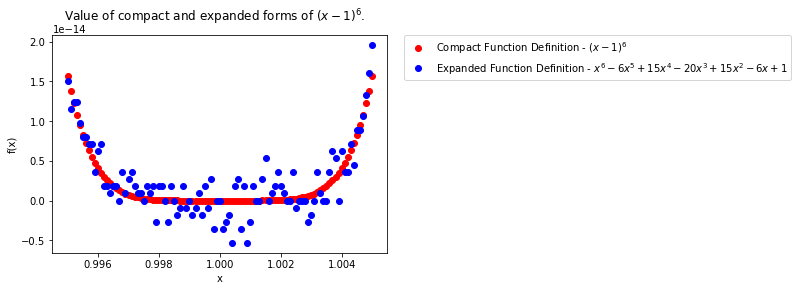
\includegraphics[width=\textwidth]{polinomial_error.png} 
	\label{fig:q10CP}
	\caption{The value of the different representations of $(x-1)^6$
	plotted over the range $[0.995, 1.005]$.}
\end{figure}

There are multiple reasons why this issue is occuring in this circumstance.
The first is that there are more opportunities for cancelation, because there
are more subtractions in the function. The second, and probably the more important
one, is that for values so close to one, the higher powers in the expanded terms are
driven very close to 1, so the cancelation that happens in these terms is much more severe.
In the compact term, the cancelation is minimal, because the subtraction occurs
when the values have not been pulled close together, so the cancelation isn't bad.
Then with this relatively unpertubed value, we take the sixth power,
which doesn't cause much error.



\section{Chapter 2}
\subsection{Exercises}
\subsubsection{Question 2.7}
We have the matrix $A = 
\bigl( \begin{smallmatrix} 
  1 & 1 + \epsilon\\
  1 - \epsilon & 1 
\end{smallmatrix} \bigr)$

\textit{(a)}
The determinant of this matrix is
$$1 - (1 + \epsilon) * (1 - \epsilon)$$
$$= 1 - 1 + \epsilon - \epsilon + \epsilon^2$$
$$ = \epsilon^2$$

\textit{(b)}
The value of epsilon is the value of the machine's epsilon.
In floating point, the value of $\epsilon$ must be less than
the square root of the machine epsilon value. More formally the
required condition is
$$\epsilon < \sqrt{\epsilon_{machine}}$$

\textit{(c)}
In order to get $A$ into upper triangular, we need to annihilate the first
entry of the second row, which we do by subtracting $(1-e) *$ the first row
from the second row.

$$A = \bigl( \begin{smallmatrix}
		   1 & 0\\
    	   -(1 - \epsilon) && 1
           \end{smallmatrix} \bigr)
           * \bigl( \begin{smallmatrix} 
			  1 & 1 + \epsilon\\
  			  1 - \epsilon & 1 
			\end{smallmatrix} \bigr)
		= \bigl( \begin{smallmatrix} 
			  1 & 1 + \epsilon\\
  			  0 & \epsilon^2 
			\end{smallmatrix} \bigr) = LU$$
			
so $L =\bigl( \begin{smallmatrix} 
			  1 & 1 + \epsilon\\
  			  1 - \epsilon & 1 
			\end{smallmatrix} \bigr)$
and $U = \bigl( \begin{smallmatrix} 
			  1 & 1 + \epsilon\\
  			  0 & \epsilon^2 
			\end{smallmatrix} \bigr).$
			
\textit{(d)}
The determinant of A and U are the same, so the same thing must hold
in order for U to be singular (i.e. the determinant be 0).

$$\epsilon < \sqrt{\epsilon_{machine}}$$

\subsubsection{Question 2.13}
First solve the lower triangular system $L_1 x = b$ for x by forward substitution. Then
solve the lower triangular system$L_2 y = x - Bx$ for y by using forward substitution.

{
\color{red} I PROMISE I'LL DO IT!
}

\subsubsection{Question 2.21}
$$x = B^{-1} (2A + I)(C^{-1} + A)b$$

Let's go right to left. First thing is first, we can compute $x = Ab$, as well as
solve out the inverted C matrix which is giving us trouble by setting $Cy = b$ and
solving for $y$. We then have

$$x = B^{-1} (2A + I)(y + x)$$

let's combine x and y to give us z, so $z = x + y$.
$$x = B^{-1} (2A + I)z$$

The rightmost term can be called $w  = (2A + I) z$ we now have
$$x = B^{-1} w.$$

Finally we solve the equation $Bx = w$ for x and we have our result for x without
inverting any matrices.

\subsubsection{Question 2.22}

We are factorizing an \textbf{n by n} matrix. The reduction of the matrix into L and U
by Gaussian Elimination requires, at each row \textbf{i}

\begin{enumerate}
\item The selection of the annihilation value for each of the $n-i$ rows below.
\item The multiplication of the current row by each of these factors and the subsequent subtraction 
of these scaled values from the below rows in the U matrix. This is the annihilation step.
\item The matrix multiplication of the current culmulative L by the annihilating opperation matrix. This I'll call the accumulation step.
\end{enumerate}

For the following complexity assume the matrices are indexed starting at 1.

\begin{flushleft}
\begin{tabular}{c | c}[H]

Step & Approximate Complexity (size n and current row i)\\
\hline
Selection & n - i (only multiplications)\\
Annihilation & $(n-i + 1)(n-i)$ (both multiplications and subtractions)\\
Accumulation & {\color{red}I can't figure out the complexity.}\\
\end{tabular}
\end{flushleft}

The first step is negligible in terms of complexity. The second step is by far the dominant
step in terms of complexity. We have effectively $(n-i+1)(n-i)$ multiplications and
subtractions at step i with a matrix of size n.

Over the whole process, we then have

$$\sum_{i=1}^{i=n}(n-i+1)(n-i) \approx \sum_{i=1}^{i=n}(n-i+1)^2 = \sum_{i=1}^{i=n}i^2 = 
\frac{n(n+1)(2n+1)}{6}$$

therefore the dominant term is the $\frac{2n^3}{6}$ term which reduces to $$\frac{n^3}{3}.$$

\subsubsection{Question 2.32}
We need to show that the following functions satisfy the first three properties of a matrix norm.

\textit{The matrix norms we have defined satisfy the following important properties, 
where A and B are any matrices:
\begin{enumerate}
\item $\lvert \lvert A \rvert \rvert > 0$ if $A \neq O$.
\item $\lvert \lvert \gamma A \rvert \rvert = \lvert \gamma \rvert * \lvert \lvert A\rvert 
\rvert$ for any scalar $\gamma$.
\item $\lvert \lvert A + B \rvert \rvert \leq \lvert \lvert A \rvert \rvert + \lvert \lvert B 
\rvert \rvert$.
\end{enumerate}
}

\textit{(a)} The norm is given:
$$ \lvert \lvert A\rvert \rvert_{max} = \max\limits_{i,j} \lvert a_{i,j}\rvert $$

\textit{(i)} If $A \neq 0$ then some $a_{ij} \neq 0$ so $\lvert a_{ij}\rvert > 0$
therefore
$$\max\limits_{i,j} \lvert a_{i,j}\rvert > 0 \quad if \quad A \neq 0.$$


\textit{(ii)} For the second condition:
$$\lvert \lvert \gamma A \rvert \rvert_{max} = \max_{i,j}\lvert \gamma a_{ij} \rvert
= \lvert \gamma\rvert \max_{i,j} \lvert a_{ij} \rvert
= \lvert \gamma\rvert * \lvert \lvert A \rvert \rvert_{max}$$

\textit{(iii)} Finally we have for the third condition, with matrices $A$ and $B$
let's assume we have the following:
$$\lvert \lvert A\rvert \rvert_{max} = \lvert a_{i,j} \rvert$$
$$\lvert \lvert B\rvert \rvert_{max} = \lvert b_{k,l} \rvert$$

The most agressive case would be if $a_{i,j}$ and $b_{k,l}$ are the same sign.
In this case we have
$$\lvert \lvert A + B \rvert \rvert_{max} = \lvert a_{i,j} + b_{k,l} \rvert 
= \lvert a_{i,j} \rvert + \lvert b_{k,l} \rvert
= \lvert \lvert A \rvert \rvert_{max} + \lvert \lvert B \rvert \rvert_{max}$$

This is the equality case, and it is a true equality, that is scaling either
of the max values leads to the same increase in the norm of the combination.

If the signs are flipped (i.e the elements which have the largest absolute value in
both A and B are opposite sign) then we cannot possibly have equality, and we've
already shown that we can't go above equality, so we must have a smaller value in
the combined norm than in the sum of the two seperate norms.

{\color{red} This is a shitty explanation for the last part. Do a better job.}

\textit{(b)}
$$ \lvert \lvert A\rvert \rvert_{F} = \left( \sum_{i,j}\lvert a_{i,j} \rvert^{2} \right)^{\frac{1}{2}} $$

{\color{red} I CAN'T DO THIS RIGHT NOW.}


\subsubsection{Question 2.37}

$$B = \left[ \begin{smallmatrix} \alpha & a^{T} \\ a & A \end{smallmatrix} \right]$$
{\color{red}
\textit{(a)}

\textit{(b)}
}


\subsection{Computer Exercises}
\subsubsection{Question 2.5}
\subsubsection{Question 2.6}
\subsubsection{Question 2.9}
\subsubsection{Question 2.11}
\subsubsection{Question 2.17}
\end{document}
